\chapter{Testbed - Prototype Implementation}
\label{chap:referenceimplementation}

As already discussed in chapter \ref{chap:introduction}, sensing a city's parking availability and thus making the parking situation more transparent would be highly beneficial for reducing traffic congestion and greenhouse gas emissions as driver's looking for parking spaces in urban areas could navigate directly to vacant parking spaces close to their destinations. In this thesis a prototype of drive-by sensing using an optical distance sensor has been designed, implemented and evaluated. This chapter discusses the test bed which has been developed to acquire the necessary dataset to run the machine learning experiments as well as the process to obtain ground truth information.

%This chapter will describe the setup and implementation of the prototype. In particular, section \ref{sec:system_design} will discuss the overall envisioned system, the prototype car and the required sensors with their capabilities. In section \ref{sec:experiment_description_data_collection} the experimental setup will be discussed as well as the acquiring of the test dataset through test drives in the city of Linz, Austria. Finally, section \ref{sec:data_processing} will describe the preprocessing of the data, definition of the features and a short description of all used machine learning algorithms with their configurations. 
%\todo{update :)}




%\section{System design}
%\label{sec:system_design}


%\begin{description}
%
%
%\item[Building a test bed] As a first step a test bed has to be built which is able to access the required sensors to record all the necessary data. A Raspberry Pi will be used as processing device because of its popularity and the many compatible sensors which work with this platform. It is connected to a LIDAR-Lite v3 sensor which continuously measures the distance to the nearest obstacle on the right side of the road. A GPS receiver will track the location of the sensing vehicle and a camera will be used to record images of the ground truth for evaluation purposes only. In section \ref{sec:system_design} the complete setup of the test bed is described as well as all the specific hard ware parts and their abilities.
%
%\item[Acquiring a dataset] As soon as the test bed is ready, the sensors should be mounted on the prototype car to be able to start recording the dataset. Test drives should be done in some selected streets in Linz, Austria with the focus of variety of the recorded situations. The test scenes should include single lane as well as multi lane streets and measurements in all streets should be done several times. Furthermore, the car should be driving as it would in regular traffic (not only in the right most lane, etc...) and the scenes should also include high and low traffic scenarios to have a high amount of diverse data. All measured distances, GPS locations and ground truth images have to be saved to files with the according timestamps to be able to evaluate the results of different approaches later on. Furthermore, using the images taken by the camera, ground truth values will be manually labelled in different classes (Parked car, free space, overtaken car, ...). A detailed description about the dataset and the ground truth tagging can be found in section \todo{ref} \ref{sec:dataset}.
%
%\item[Data processing and segmentation] As next step the measured sensor values have to be preprocessed and filtered in order for the following algorithms to work. Sensing and overflow errors as well as outliers in the measurements should be identified and removed before further processing. After the raw data has been filtered, the sensor data has to be segmented. As parking cars and other cases which should be classified consist of several sensor measurements, the corresponding sensor measurements should be grouped together and merged to segments which will be later classified. All preprocessing steps and the segmentation process are described in more detail in section \todo{ref} \ref{sec:data_processing}.
%
%\item[Classification using basic machine learning techniques] Features on the created segments are calculated (for instance length, average distance and variation of the distances) and are being used to train and evaluate several machine learning algorithms which will be compared on their performance. Furthermore, some deep learning models will also be evaluated on the raw sensor data of the segments and will be compared to common machine learning results. The results of all experiments can be found in section \todo{ref} \ref{sec:ml_results}.
%
%\item[Further improvements] \todo{todo}
%
%\end{description}









\section{Used Hardware and Sensor Parts}
\label{sec:test_bed}

Figure \ref{fig:sensing_car} shows the sensing car and its mounted sensors. For collecting, processing and saving the sensed data a Raspberry Pi 2 Model B\footnote{\url{https://www.raspberrypi.org/products/raspberry-pi-2-model-b/}} is being used. A Raspberry Pi was chosen because of its simplicity to connect and access sensors and moreover because it is really easy to program with it as it is just a regular linux-based computer. Furthermore, the price of a Raspberry Pi is also quite low (about \euro{35}), therefore the overall cost of the system will remain low.


\begin{figure}
	\centering
	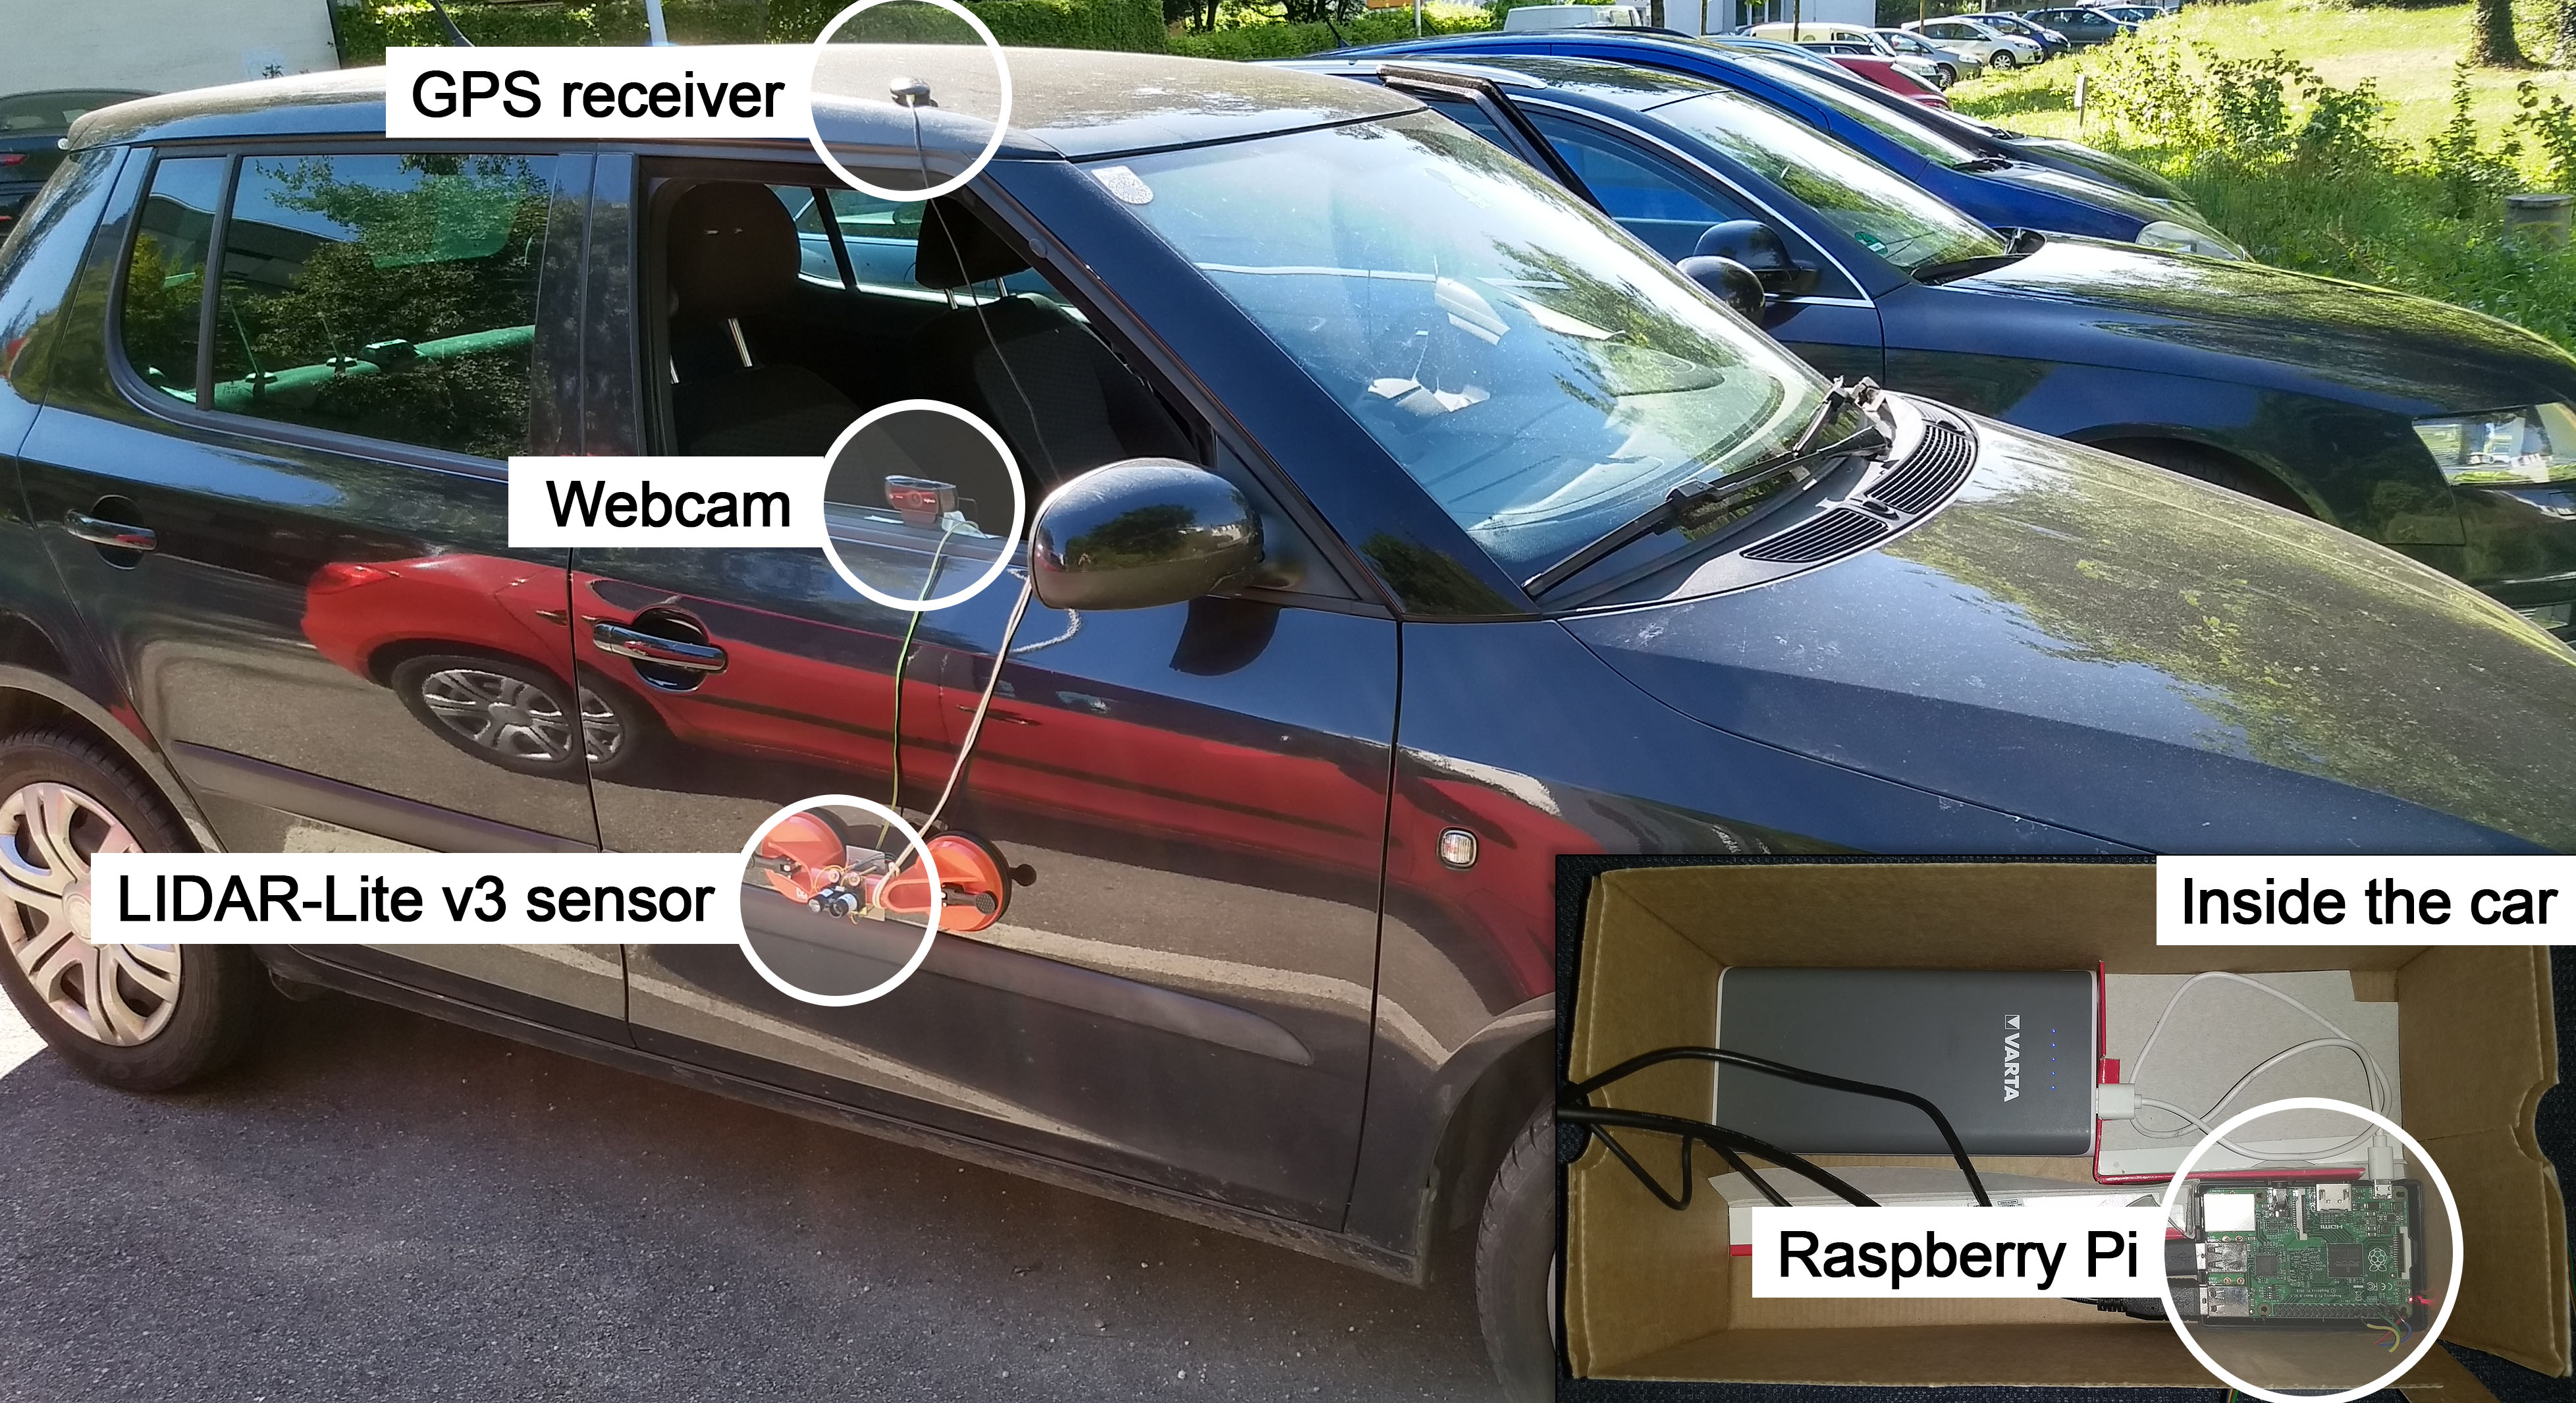
\includegraphics[width=\textwidth]{img/car.jpg}
	\caption{Prototype of the sensing car, which is composed of a LIDAR Lite v3 optical distance sensor, a GPS receiver, a camera for ground truth collection and a Raspberry Pi as processing device}
	\label{fig:sensing_car}
\end{figure}


To determine the location of the sensing vehicles while driving through the city, a Navilock USB GPS receiver\footnote{\url{http://www.navilock.de/produkte/G_61840/merkmale.html?setLanguage=en}} is being used. It can be connected to the Raspberry Pi using a USB Port and can measure the GPS location (latitude and longitude) at a rate of about 1 Hz. According to the manufacturer the acquired positions are correct in the range of 2.5 meters. The GPS receiver is mounted on the top of the sensing car using a magnet which should help to receive more accurate sensor readings. The Navilock USB GPS sensor starts at a price of about \euro{50}.

For the use of a distance sensor there are two options. Either a ultrasonic range sensor can be used or an optical laser distance sensor. While ultrasonic sensors are cheap and widely used in commercial parking assistance systems, they also have limitations in terms of sensing frequency (about 20 Hz) and range (a few meters). These specifications limit the use of ultrasonic sensors for using drive-by sensing on multi-lane roads or with high speeds. Due to these limitations the optical distance sensor "Lidar Lite v3\footnote{\url{https://www.sparkfun.com/products/14032}}" is being used. It measures the time of flight of an emitted laser signal which is reflected by an object in its way. The Lidar Lite v3 can measure distances from a few centimeters up to 40 meters at a frequency of 1 to 500 Hz. Furthermore, it is able to measure distances with an accuracy of about 2.5 centimeters. However, in comparison to ultrasonic sensors, optical sensors are more expensive. While ultrasonic sensors can be bought under \euro{10}, the Lidar Lite v3 and other comparable sensors are about \euro{150}.

The distance sensor is mounted on the co-driver's door using a sucker handle, so that it faces to the right side of the road and so that it measures about \todo{40cm} above the ground. Moreover, it is connected to the Raspberry Pi via GPIO (General Purpose Input Output) pins while communicating using an I2C (Inter Integrated Circuit) interface, according to the manufacturer's specifications.

Table \ref{table:comparison_us_lidar} shows a comparison of the capabilities of ultrasonic sensors and our used Lidar Lite v3 sensor. The most significant limitation is the sampling frequency. While optical laser sensors are based on the speed of light, ultrasonic sensors are based on the speed of sound, which is much slower. Therefore, also the distances between consecutive measurements varies highly from an ultrasonic to an optical laser sensor. At a speed of 50 km/h, a sensing vehicle would drive up to 70 cm between two consecutive measurements with an ultrasonic sensor while only driving about 3 cm when using an optical distance sensor.



\begin{table}


\resizebox{\textwidth}{!}{%
\bgroup
\def\arraystretch{1.4}
\begin{tabular}{| r || c | c |}
\hline
   & 
   \textbf{Ultrasonic Range Finder} & 
   \textbf{Lidar Lite v3} \\
%\hline
\hline
  \textbf{Costs} & 
   from about \euro{5,00} to \euro{100,00} &
   about \euro{150,00} \\
\hline
  \textbf{Sampling Frequency} & 
   up to 20 Hz &
   up to 500 Hz \\
   & (at 10 m distance) & \\
\hline
  \textbf{Range} & 
   2 cm - 10 m &
   30 cm - 40 m \\
\hline
  \textbf{Distance between Measurements} & 
   about 70 cm &
   about 3 cm \\
  \textbf{at 50 km/h} & & \\
\hline

\end{tabular}
\egroup
}

\caption{Comparison of ultrasonic sensors and the used Lidar Lite v3 optical distance sensor}
\label{table:comparison_us_lidar}
\end{table}

For the camera which is necessary to capture images of the ground truth a Logitech C922 Pro Stream\footnote{\url{https://www.logitech.com/en-us/product/c922-pro-stream-webcam}} is being used. At a frequency of about 30 Hz images with a resolution of 352 x 288 pixels are captured while the car is sensing parking spaces. The camera is mounted on the co-driver's door on the same horizontal position as the sensor. This way the center of the image will be the position where the distance sensor is measuring its distances. The Logitech camera is connected to the Raspberry Pi using an USB Port and is available at about \euro{90}.





%\begin{table}
%
%\bgroup
%\def\arraystretch{1.5}
%\begin{tabular}{| r || c | c |}
%\hline
%   & 
%   \textbf{Sampling Frequency} & 
%   \textbf{Costs per Sensor} \\
%%\hline
%\hline
%  \textbf{Lidar Lite v3} & 
%   ~200 measurements/s &
%   \euro{169,00} \\
%\hline
%  \textbf{Navilock USB} & 
%   ~1 measurement/s &
%   \euro{74,90} \\
%   \textbf{GPS receiver} & & \\
%\hline
%
%\end{tabular}
%\egroup
%
%\caption{The used sensors}
%\label{table:sensors_capabilities}
%\end{table}


\section{Collecting Sensor Measurements}
\label{sec:sensor_measurement_collection}

A python script has been developed which saves all sensor readings during the test runs into a text file for later analysis and evaluation. Furthermore, all images captured by the camera are saved into a specific folder on the Raspberry Pi to be able to derive the ground truth information later on.
%To collect the sensor readings while the sensing vehicle is driving a python script was developed which saves all sensor readings to a text file and the images captured by the camera into a specific folder on the Raspberry Pi.
The sensing of all three devices (GPS, Lidar Lite v3, Logitech camera) runs asynchronously in separate threads so that none of them influence the other sensor's readings. For accessing the GPS receiver the python gps library was used whereas for measuring the distance using the Lidar Lite v3 sensor, an open source library available on github.com was used (\url{https://github.com/Sanderi44/Lidar-Lite}). 
%A library called "pygame.camera" was used to capture the images of the webcam. 

Figure \ref{fig:sample_sensor_trace} shows a part of a sensor trace which was acquired during a test drive. It contains GPS and distance measurements. The first column determines which sensor was used for the specific measurement and the second one is the time stamp of the Raspberry Pi's system time in seconds. GPS measurements also show latitude, longitude and speed measurements while the Lidar Lite measurements only show the measured distance in centimeters.

%\begin{figure}
%	\centering
%	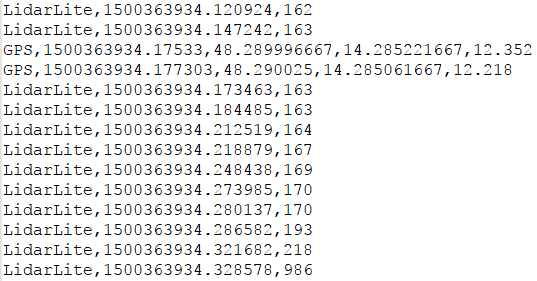
\includegraphics{img/sample-sensor-trace.PNG}
%	\caption{Sample of the collected sensor trace}
%	\label{fig:sample_sensor_trace}
%\end{figure}

\begin{figure}
	\centering
	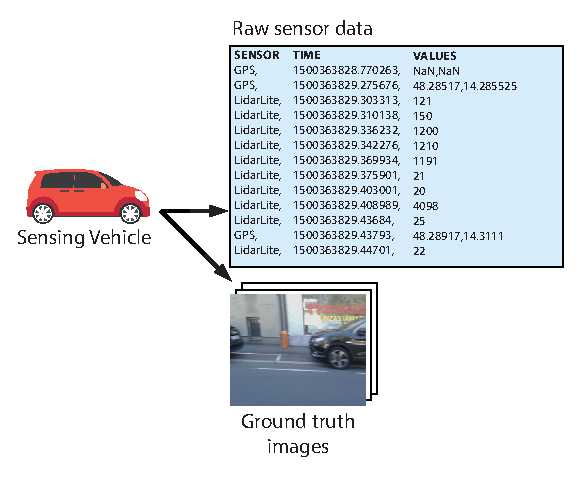
\includegraphics{img/obtaining-raw-dataset.eps}
	\caption{Sample of the collected sensor trace}
	\label{fig:sample_sensor_trace}
\end{figure}



\section{Raw Dataset}
\label{sec:raw_dataset}

%As soon as the test bed is ready, the sensors should be mounted on the prototype car to be able to start recording the dataset. Test drives should be done in some selected streets in Linz, Austria with the focus of variety of the recorded situations. The test scenes should include single lane as well as multi lane streets and measurements in all streets should be done several times. Furthermore, the car should be driving as it would in regular traffic (not only in the right most lane, etc...) and the scenes should also include high and low traffic scenarios to have a high amount of diverse data. All measured distances, GPS locations and ground truth images have to be saved to files with the according timestamps to be able to evaluate the results of different approaches later on. Furthermore, using the images taken by the camera, ground truth values will be manually labelled in different classes (Parked car, free space, overtaken car, ...). A detailed description about the dataset and the ground truth tagging can be found in section \todo{ref} \ref{sec:dataset}.

To obtain a dataset, in total 32 test drives were completed in the city of Linz, Austria. The sensed street scenarios have been selected with the focus of variety of the recorded situations. The test scenes include single lane as well as multi lane streets and measurements in all streets have been done several times. Furthermore, while collecting the test measurements the sensing car was driving as it would in regular traffic (not only in the right most lane, etc.) and the scenes also include high and low traffic scenarios to have a high amount of diverse data. 
Figure \ref{fig:gps_locations_dataset} shows an aggregated GPS trace of all test drives on a map of Linz. Red dots represent parking cars while black dots represent other objects. In total 444.427 distance measurements and 14.997 GPS measurements were taken, which makes up about 15,9 megabytes of distance and GPS data. 
Additionally, 266.309 images were captured to record the ground truth of the sensed scenes. All of these images which make up about 5.072 megabytes are used to determine the ground truth of the recorded scenes to be later able to apply supervised machine learning. How ground truth tagging was done is described in the following section.



\begin{figure}
	\centering
	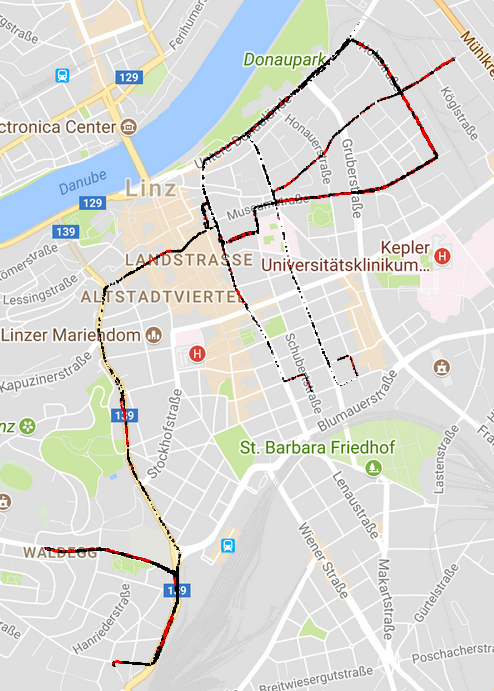
\includegraphics{img/gps_data_recorded_data_parking_spaces.PNG}
	\caption{GPS Trace of all recorded samples in the acquired dataset, while 32 test drives in Linz, Austria. Red dots represent parking cars.}
	\label{fig:gps_locations_dataset}
\end{figure}




\section{Ground Truth Tagging}
\label{sec:ground_truth_tagging}

The recorded raw dataset contains distance and position measurements as well as images showing the ground truth at a specific time stamp. To be able to process the ground truth information included in the images, a manual ground truth tagging task has to be performed. Figure \ref{fig:ground_truth_tagging_ui} shows the user interface of the program which was implemented to manually tag an image with one of nine pre selected class labels. The user first has to select the directory with the captured images. The file name of each image is the time stamp when it was recorded, therefore this information is known. When the images are loaded, the user has to tag the situation which is present at the red line, which demonstrates the center of the picture. For instance, figure \ref{fig:ground_truth_tagging_ui} shows a parking car at the center of the image. Moreover, on the right of the image a car which has been overtaken by the sensing vehicle is also visible.
The class labels of which the user can choose are the following:

\begin{figure}
	\centering
	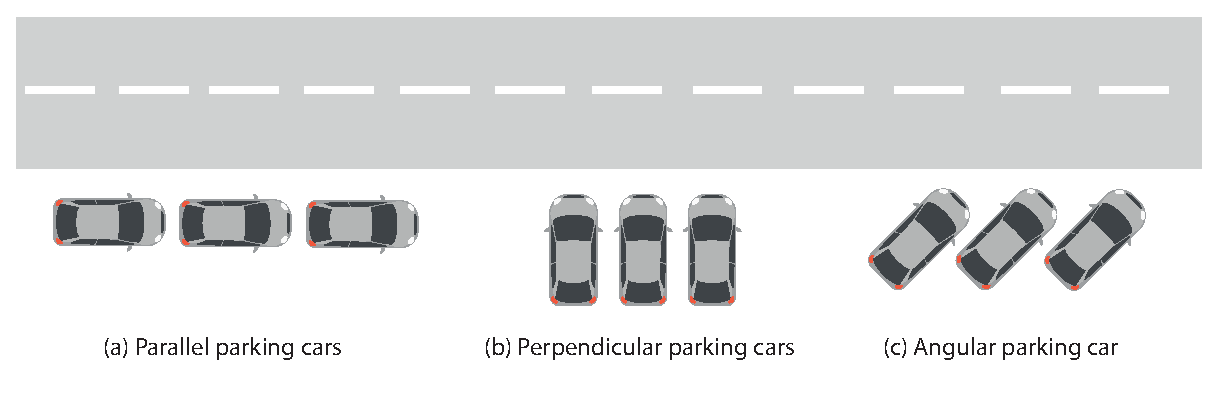
\includegraphics[width=\textwidth]{img/types-of-parking-cars.eps}
	\caption{Different types of parking cars}
	\label{fig:types_of_parking_cars}
\end{figure}

\begin{description}

\item[Parking car] A non-moving vehicle which is parking at the right side of the road. There are three kinds of parking vehicles from which one can choose: Parallel parking cars, perpendicular parking cars and angular parking cars. Figure \ref{fig:types_of_parking_cars} shows the different types of parking spaces.

\item[Overtaking Situation] This class label means that the sensing vehicle is overtaking another traffic participant. The user can choose between overtaken cars, overtaken motorcycles and overtaken bicycles.

\item[Other parking vehicle] The user can tag parking motorcycles and parking bicycles which also should be detected later on. This class represents obstacles which can be located on parking spaces and therefore make it unavailable for parking.

\item[Free space] This class label should be used, when none of the above listed class labels are applicable. It represents a free space where it is maybe possible to park a vehicle. Yet only with the help of a parking space map, a free space can be marked as vacant parking space as a random free space may be an illegal parking space.

\end{description}



The output of the ground truth tagging process is written into a text file where each line represents an entry of a time stamp and its corresponding tagged ground truth class label. This ground truth file will be further processed in the next steps which will be discussed in the following sections.





\begin{figure}
	\centering
	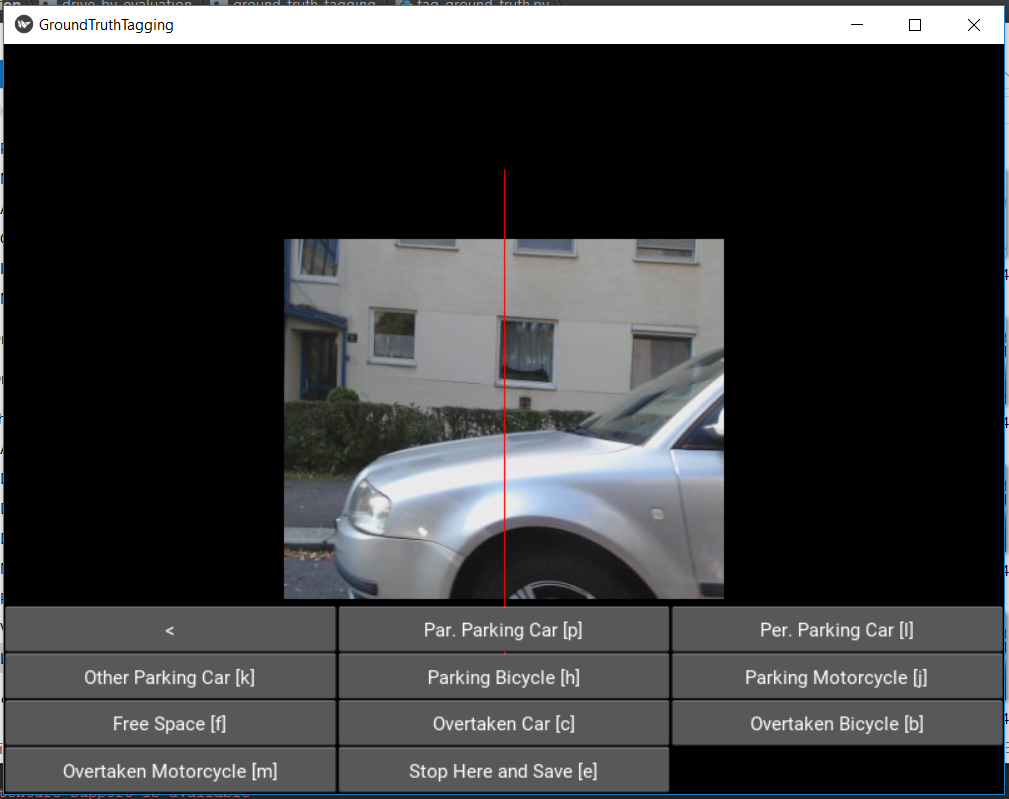
\includegraphics[width=0.8\textwidth]{img/ground_truth_tagging_ui.PNG}
	\caption{User Interface to manually tag what kind of situation is faced during the specific time the image shown is taken}
	\label{fig:ground_truth_tagging_ui}
\end{figure}



\section{Data Preprocessing}

Before the raw dataset can be used for the input of machine learning models, a few preprocessing steps have to be taken. First of all, error values of the GPS sensor and the LiDAR Lite v3 sensor are thrown away. The GPS sensor usually shows erroneous output (NaN values) when it starts sensing due to the fact that it is not yet connected to enough satellites. The distance sensor can provide overflow measurements when the target object is too far away or too close to the sensor. In both cases it will give an output of less than 10 centimeters. All of the detected error/overflow measures will be simply deleted from the raw dataset before further processing to ensure the quality of the data.

Due to the fact that all sensors measure at different frequencies, the sensor data of all sensors has to be unified before the next steps can be taken. The distance sensor measures at a much higher frequency than both the GPS sensor and the camera. Therefore, the GPS location as well as the ground truth at each distance measurement have to be approximated. Linear interpolation using the timestamp of the measurements is being used to calculate the approximate location and ground truth at the times of all distance measurements. Figure \ref{fig:preprocessing_dataset} shows how the raw sensor data and the ground truth data get unified so that a list of data points containing distance, GPS position and ground truth can be derived.

\begin{figure}
	\centering
	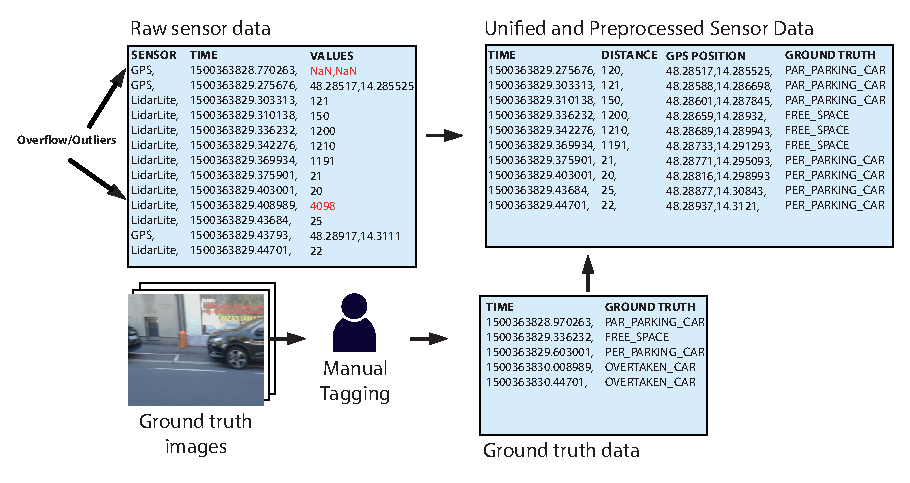
\includegraphics[width=\textwidth]{img/dataset-preprocessing.eps}
	\caption{All sensor measurements are being merged to obtain samples with time, distance, location and ground truth information}
	\label{fig:preprocessing_dataset}
\end{figure}





\section{Data Segmentation}

As the used distance sensor measures at a high frequency, it usually collects several distance measurements belonging to the same object. For example, if the sensing vehicle passes a parallel parked car (having a length of 4 meters) at a speed of 30km/h it will collect approximately 24 measurements belonging to the passed car. To be able to automatically evaluate the performance of different approaches to sense parking cars and other objects the sensor measurements belonging to the same objects have to be grouped together. After the raw dataset has been collected and the ground truth has been tagged, this operation, called segmentation, is being performed.




\begin{figure}
	\centering
	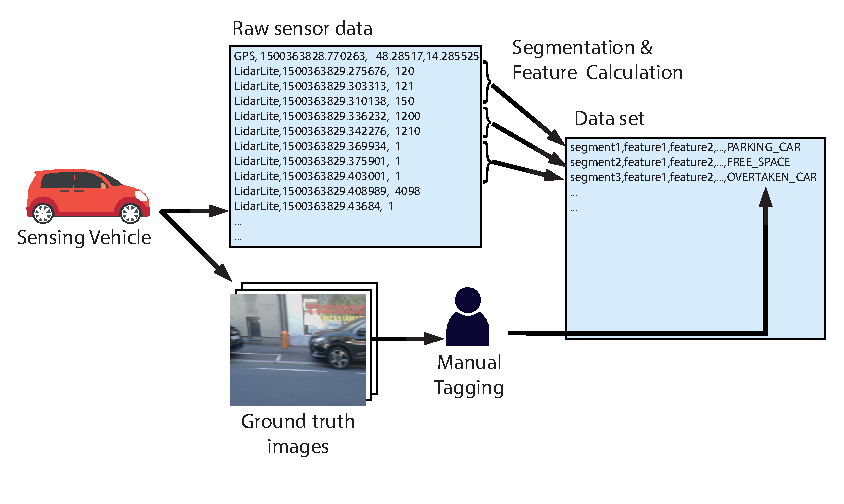
\includegraphics[width=\textwidth]{img/obtaining-dataset-architecture.eps}
	\caption{Steps to obtain the dataset from the raw sensor measurements and ground truth recordings}
	\label{fig:dataset_architecture}
\end{figure}







\chapter{Data Processing and Machine Learning Approaches}

\section{Experiment description and data collection}
\label{sec:experiment_description_data_collection}
- Description of experiments (scenarios we are interested in: parking car, etc.)
- Data set derived (raw data, size, etc.)
- Map data and camera ground truth data



\section{Data processing}
\label{sec:data_processing}
- Preprocessing, feature definition ...
- Traditional ML Algorithms (incl. a short description of each algorithm and configuration options)
- Deep Learning